\section{Introduction}
\label{sec:intro}

\subsection{Motivation}

A Water Quality Index (WQI) condenses a panel of physical, chemical and biological measurements into one number and one category, so that a river reach can be called ``good'' or ``poor'' by people who will never read a laboratory sheet. It is the standard way Indian and international agencies communicate river condition to the public and to decision-makers~\citep{horton1965,brown1970,tyagi2013,uddin2021}. The difficulty is that a WQI is only as available as its \emph{full} parameter panel. Several of the panel's inputs are slow or expensive: biochemical oxygen demand (BOD) needs a five-day incubation, coliform counts need 24--48\,h of culturing, and nutrients need laboratory chemistry. A station that misses any one of them on a given visit cannot report a WQI for that visit.

This is not a hypothetical problem. In the Central Pollution Control Board (CPCB) National Water Quality Monitoring Programme (NWMP) river data analysed here, only \textbf{14.7\%} of the 32,968 river monitoring visits between 2018 and 2021 report all eight parameters needed for the index. In contrast, \textbf{75.8\%} report pH, dissolved oxygen (DO) and BOD (\cref{sec:data}). Most of the monitoring that actually happens is therefore already ``reduced-parameter'' monitoring, whether by design or by gap. If those reduced panels can be converted into a reliable estimate of the full-panel WQI, then the index becomes available for roughly five times as many visits. It also becomes available for stations and years that never had a full panel at all.

\subsection{Research question}

\begin{keybox}[Research question]
\emph{Can reduced-parameter monitoring provide reliable WQI prediction for data-scarce river systems?}
\end{keybox}

We make ``reliable'' operational through four sub-questions, each answered by a dedicated experiment:
\begin{enumerate}[label=\textbf{RQ\arabic*}]
  \item \textbf{Which parameters matter?} Which of the eight available parameters carry the information in the index? Does the answer depend on the method used to measure importance?
  \item \textbf{How few are enough?} How much accuracy is lost going from 8 to 7, 5, 4 and 3 parameters, and does \emph{which} parameters are kept matter more than \emph{how many}?
  \item \textbf{How little data is enough?} How does accuracy decay when the model is trained on only a few stations, and when it is applied to stations, rivers, states and seasons it has never seen?
  \item \textbf{Can the model say when not to trust it?} Do its prediction intervals hold their nominal coverage on unseen stations? How robust is it to missing readings and to field measurement noise?
\end{enumerate}

\subsection{Approach in one paragraph}

We treat the problem as \emph{surrogate modelling} (\cref{fig:surrogate}). The ground-truth index $y=g(x_1,\dots,x_8)$ is computed once, with the CPCB weighted-arithmetic formula, from the 4,861 river visits that have all eight parameters. A machine-learning model $f_S$ is then trained to predict that \emph{same} $y$ from a subset $S$ of the inputs. The target never changes; only the inputs the model may see do. This is what makes comparisons across subset sizes fair. We compare eight model families on twelve named subsets and on all 255 possible subsets. We use validation schemes that hold out whole stations, rivers, states or seasons, and add data-scarcity sweeps, calibrated prediction intervals, robustness tests and sensitivity analyses on the definition of the index itself. Finally, we apply the chosen reduced-parameter model to the roughly 20,000 real visits that lack a full panel.

\begin{figure}[t]
  \centering
  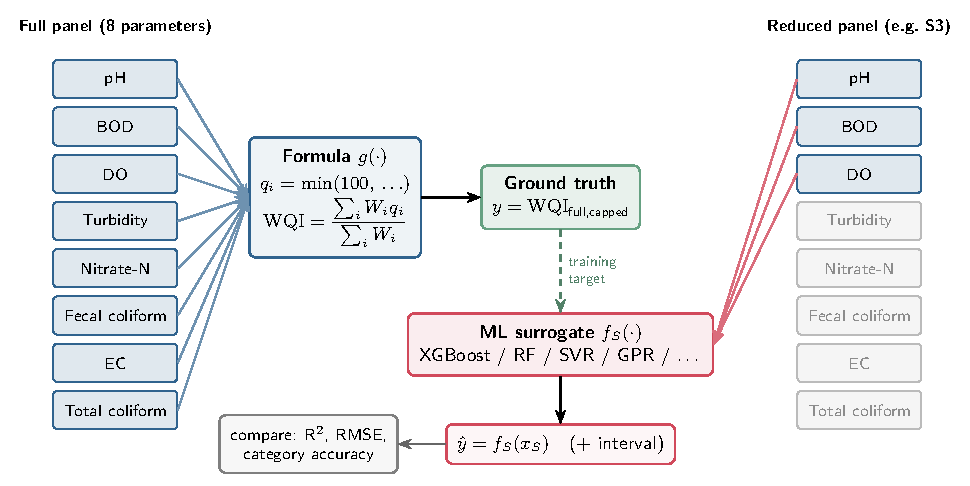
\includegraphics[width=\textwidth]{surrogate.pdf}
  \caption{The surrogate-modelling framing used throughout. The ground truth is the CPCB weighted-arithmetic WQI computed from all eight parameters (left). A model sees only a subset of the inputs (right; S3 = pH, BOD, DO shown) and is trained to reproduce the same full-panel target.}
  \label{fig:surrogate}
\end{figure}

\subsection{Contributions}

\begin{enumerate}
  \item A cleaned, audited, river-only CPCB dataset with a documented ground-truth WQI. We find that the full eight-parameter panel exists for \emph{only one year} (2020) of the 2018--2021 record (\cref{sec:data}).
  \item An exact variance decomposition of the CPCB index. It shows that the $1/S_i$ unit weights make fecal coliform, total coliform and electrical conductivity almost weightless: together they explain under 0.3\% of index variance (\cref{sec:wqi}).
  \item A consensus importance ranking from eight methods and an exhaustive search over all 255 subsets, under station-held-out validation (\cref{sec:res-importance,sec:res-subsets}).
  \item A model comparison across five validation schemes. It shows that a three-parameter model predicts the full-panel index with \R{}\,$\approx$\,0.95--0.98 at stations it has never seen, and that it clearly beats the obvious no-ML alternative of re-weighting the formula over the available parameters (\cref{sec:res-models}).
  \item Data-scarcity curves, calibrated conformal prediction intervals, and missing-data and sensor-noise robustness tests (\cref{sec:res-scarcity,sec:res-uncertainty,sec:res-robust}).
  \item Sensitivity of every conclusion to the definition of the index (standard values, equal weights, uncapped scale) (\cref{sec:res-sens}).
  \item A deployment that reconstructs full-panel WQI for about 20,000 visits that never had one, with a covariate-shift audit (\cref{sec:res-deploy}). It ends in a concrete recommended monitoring kit (\cref{sec:discussion}).
\end{enumerate}

\subsection{Organisation}

\Cref{sec:background} reviews WQI formulations and machine-learning approaches. \Cref{sec:data} describes the data and the cleaning pipeline. \Cref{sec:wqi} defines the ground truth and analyses what drives it. \Cref{sec:methods} gives the experimental methodology and \cref{sec:results} the results. \Cref{sec:discussion} answers the research question, gives the recommended kit and discusses limitations, and \cref{sec:conclusion} concludes. The appendices list hyper-parameters, full result tables and reproduction commands.
